\documentclass{article}

%%%%%%%%%%%%%%%%%%%%%%%%%%%%%%%%%%%%%%%%%%%%%%%%%%%%%%%%%%%%%%%%%%%%%%%%%%%%%%%
% Packages
%%%%%%%%%%%%%%%%%%%%%%%%%%%%%%%%%%%%%%%%%%%%%%%%%%%%%%%%%%%%%%%%%%%%%%%%%%%%%%%
\usepackage[top = 2.5cm, bottom = 2.5cm, left = 2.5cm, right = 2.5cm]{geometry}
\usepackage{mathtools}
\usepackage{amssymb}
\usepackage{soul}
\usepackage{color}
\usepackage{pdfpages}
\usepackage{graphicx}
\usepackage{setspace}
\setlength{\parindent}{0in}
\usepackage{float}
\usepackage{fancyhdr}
\usepackage{multicol}


%%%%%%%%%%%%%%%%%%%%%%%%%%%%%%%%%%%%%%%%%%%%%%%%%%%%%%%%%%%%%%%%%%%%%%%%%%%%%%%
% Header/footer
%%%%%%%%%%%%%%%%%%%%%%%%%%%%%%%%%%%%%%%%%%%%%%%%%%%%%%%%%%%%%%%%%%%%%%%%%%%%%%%
\pagestyle{fancy}
\fancyhf{}
\lhead{\footnotesize 3.R Lab: Simple Linear Regression}
\rhead{\footnotesize Pelayo, Antonio}
%\cfoot{\footnotesize  \thepage}


%%%%%%%%%%%%%%%%%%%%%%%%%%%%%%%%%%%%%%%%%%%%%%%%%%%%%%%%%%%%%%%%%%%%%%%%%%%%%%%
% Document
%%%%%%%%%%%%%%%%%%%%%%%%%%%%%%%%%%%%%%%%%%%%%%%%%%%%%%%%%%%%%%%%%%%%%%%%%%%%%%%
\begin{document}

% Title page heading 
\thispagestyle{empty}
\begin{tabular}{p{15.5cm}}
{\large \bf An Introduction to Statistical Learning} \\
{\large \bf 3.6 Lab: Linear Regression} \\
March 8, 2020\\
Antonio Pelayo \\
\hline
\\
\end{tabular}


%%%%%%%%%%%%%%%%%%%%%%%%%%%%%%%%%%%%%%%%%%%%%%%%%%%%%%%%%%%%%%%%%%%%%%%%%%%%%%%
% Section 3.6.2 Simple Linear Regression
%%%%%%%%%%%%%%%%%%%%%%%%%%%%%%%%%%%%%%%%%%%%%%%%%%%%%%%%%%%%%%%%%%%%%%%%%%%%%%%
\section*{Section 3.6.2 Simple Linear Regression} 
{\large \bf A quick look at our data}\\
We will take the time to look at the Boston housing data set in order to 
attempt to define a correlation between the median housing prices and percentage
of population that are defined as lower status. Both being quantitative data.\\

A first good step is to take a look at the plot of median housing prices against
percent lower status. This will allow us to gain initial insights to the data we
are working with.

\begin{verbatim}
> attach(Boston)
> plot(medv~lstat, 
+     xlab="Percent population in low-status",
+     ylab="Median housing price")
\end{verbatim}
\begin{figure}[!ht]
  \centering
  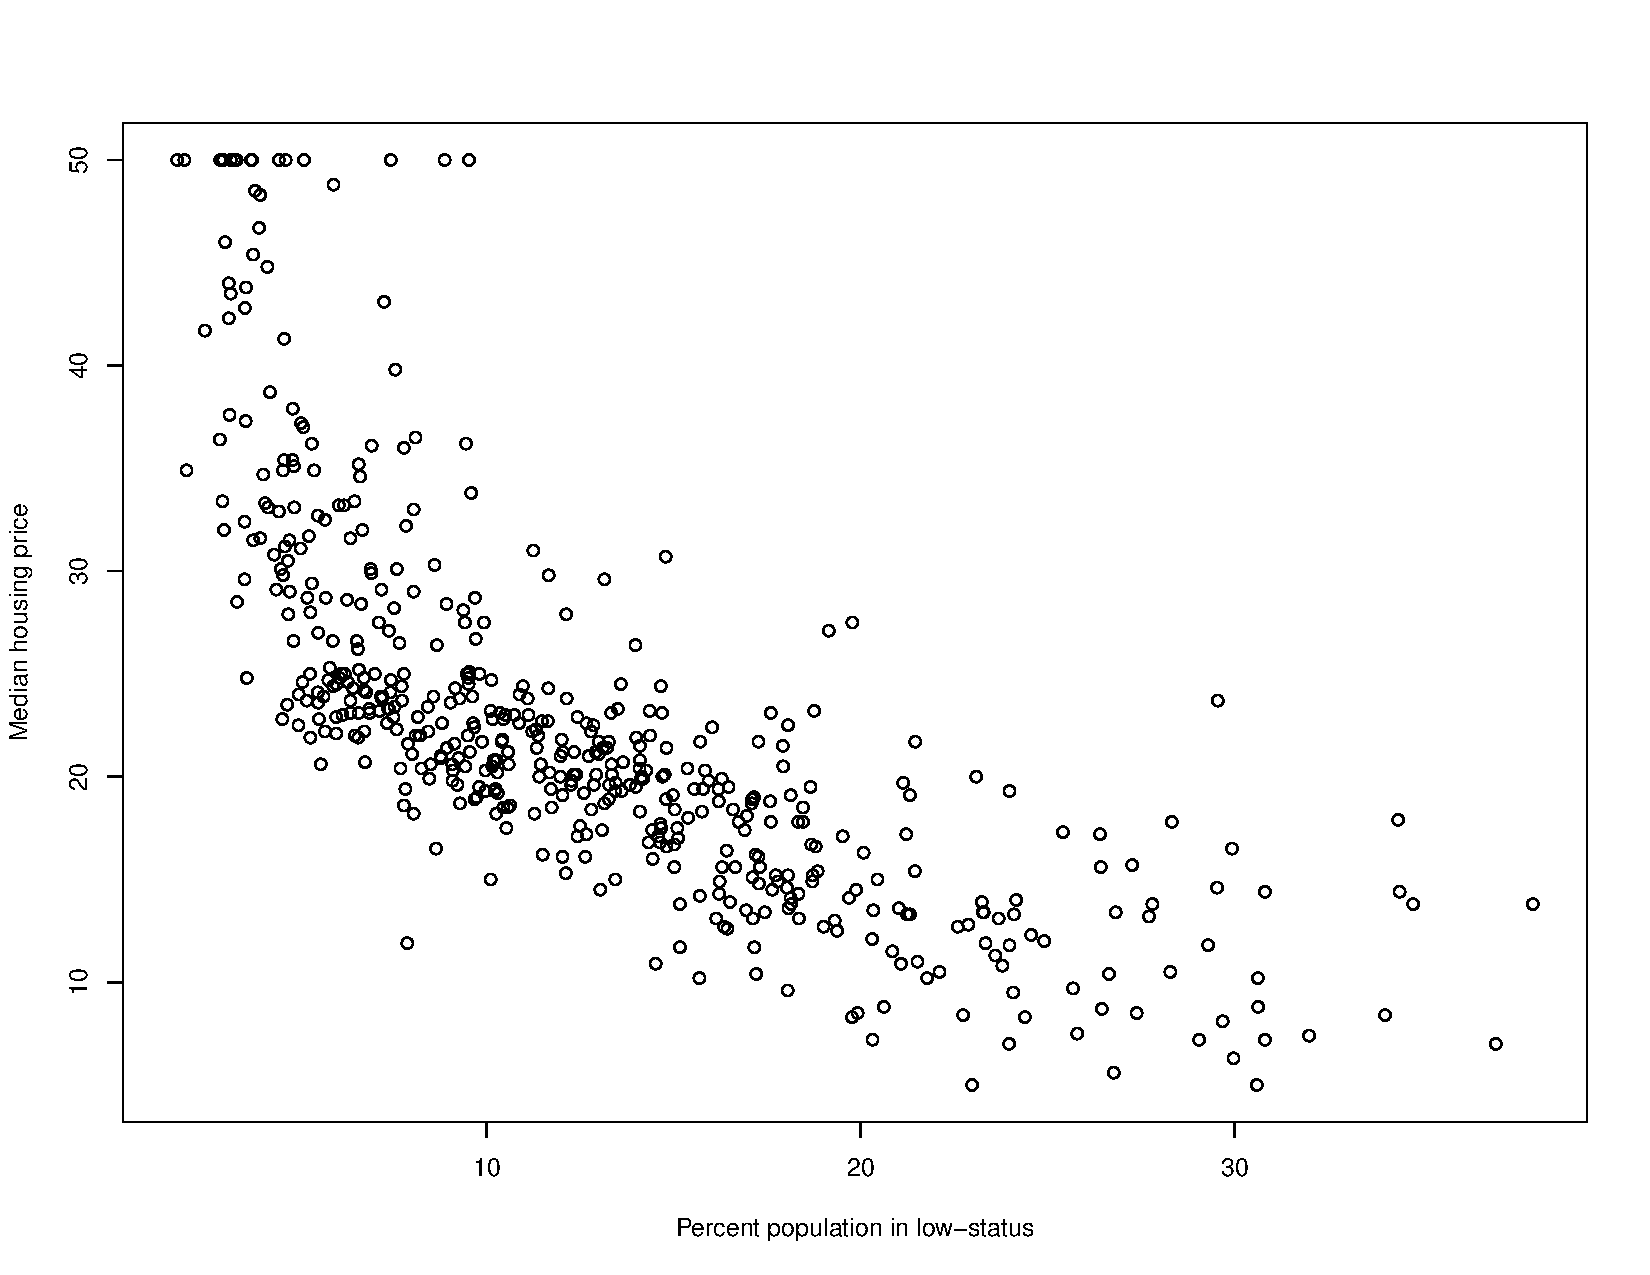
\includegraphics[width=0.65\linewidth]{medv-vs-lstat.pdf}
\end{figure}

It is possible to see that yes this graph does seem to have a general downward 
trend, though definitely not linear if we are to include all data points in 
this observation. We can use R to find 5 number summaries for these columns.

\begin{verbatim}
> summary(medv)
  Min. 1st Qu.  Median    Mean 3rd Qu.    Max. 
  5.00   17.02   21.20   22.53   25.00   50.00 
> summary(lstat)
  Min. 1st Qu.  Median    Mean 3rd Qu.    Max. 
  1.73    6.95   11.36   12.65   16.95   37.97 
\end{verbatim}

Now knowing the quartiles for our data we can compute the upper and lower fences
such that we can remove outliers in our data.

\pagebreak

%%%%%%%%%%%%%%%%%%%%%%%%%%%%%%%%%%%%%%%%%%%%%%%%%%%%%%%%%%%%%%%%%%%%%%%%%%%%%%%
{\large \bf Removing outliers}\\
\begin{align*}
  \text{Inner quartile range} &= Q3 - Q1    \\
  \text{Lower fence} &= Q1 - 1.5IQR         \\
  \text{Upper fence} &= Q3 + 1.5IQR         \\
\end{align*}

For 'medv' we have bounds at [5.05, 36.97] and for 'lstat' [-8.05, 31.95].
Applying these fences and removing the outliers we have a slightly altered graph:

\begin{verbatim}
> Boston = Boston[Boston$medv < 37 & Boston$lstat < 32,]
> plot(Boston$medv~Boston$lstat, 
+      xlab="Percent population in low-status",
+      ylab="Median housing price")
\end{verbatim}

\begin{figure}[!ht]
  \centering
  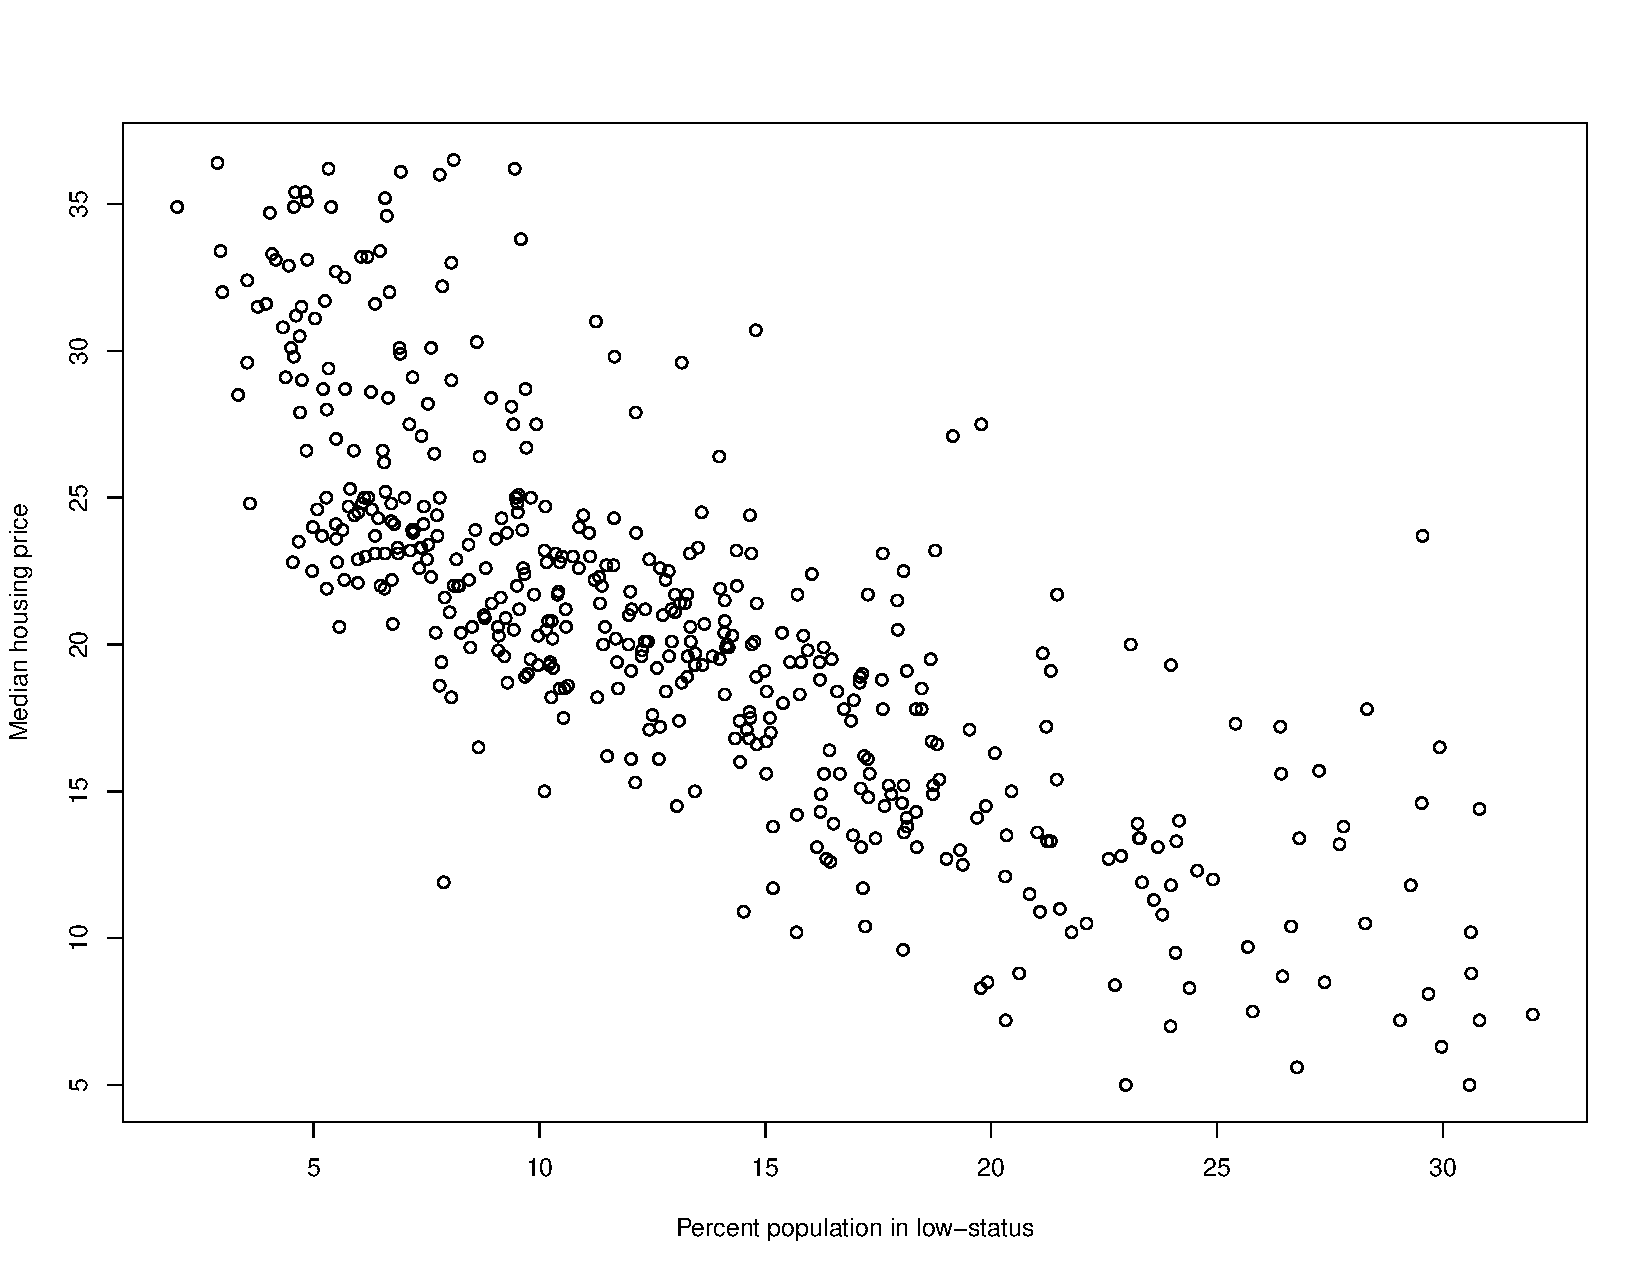
\includegraphics[width=0.65\linewidth]{medv-vs-lstat-rm-outliers.pdf}
\end{figure}


%%%%%%%%%%%%%%%%%%%%%%%%%%%%%%%%%%%%%%%%%%%%%%%%%%%%%%%%%%%%%%%%%%%%%%%%%%%%%%%
{\large \bf Applying a linear model}\\
Now we will apply a linear regression model to fit our cleaned data. 

\begin{verbatim}
> lm.fit = lm(medv~lstat, Boston)
> lm.fit    # Display regression equation coefficients

Call:
lm(formula = medv ~ lstat, data = Boston)

Coefficients:
(Intercept)        lstat  
    30.9136      -0.7785  
\end{verbatim}

This tells us that our prediction equation has values 
$\beta_0 = 30.91, \beta_1 = -0.78$

\begin{center}
  $\hat{y_i} = 30.91 - 0.78x_i$
\end{center}

It can be found through 'summary()' that the p-value for this linear model is
less than 2.2e-16, and R-squared value of 0.62 thus fitting our data fairly well.
\pagebreak

\begin{figure}[!ht]
  \centering
  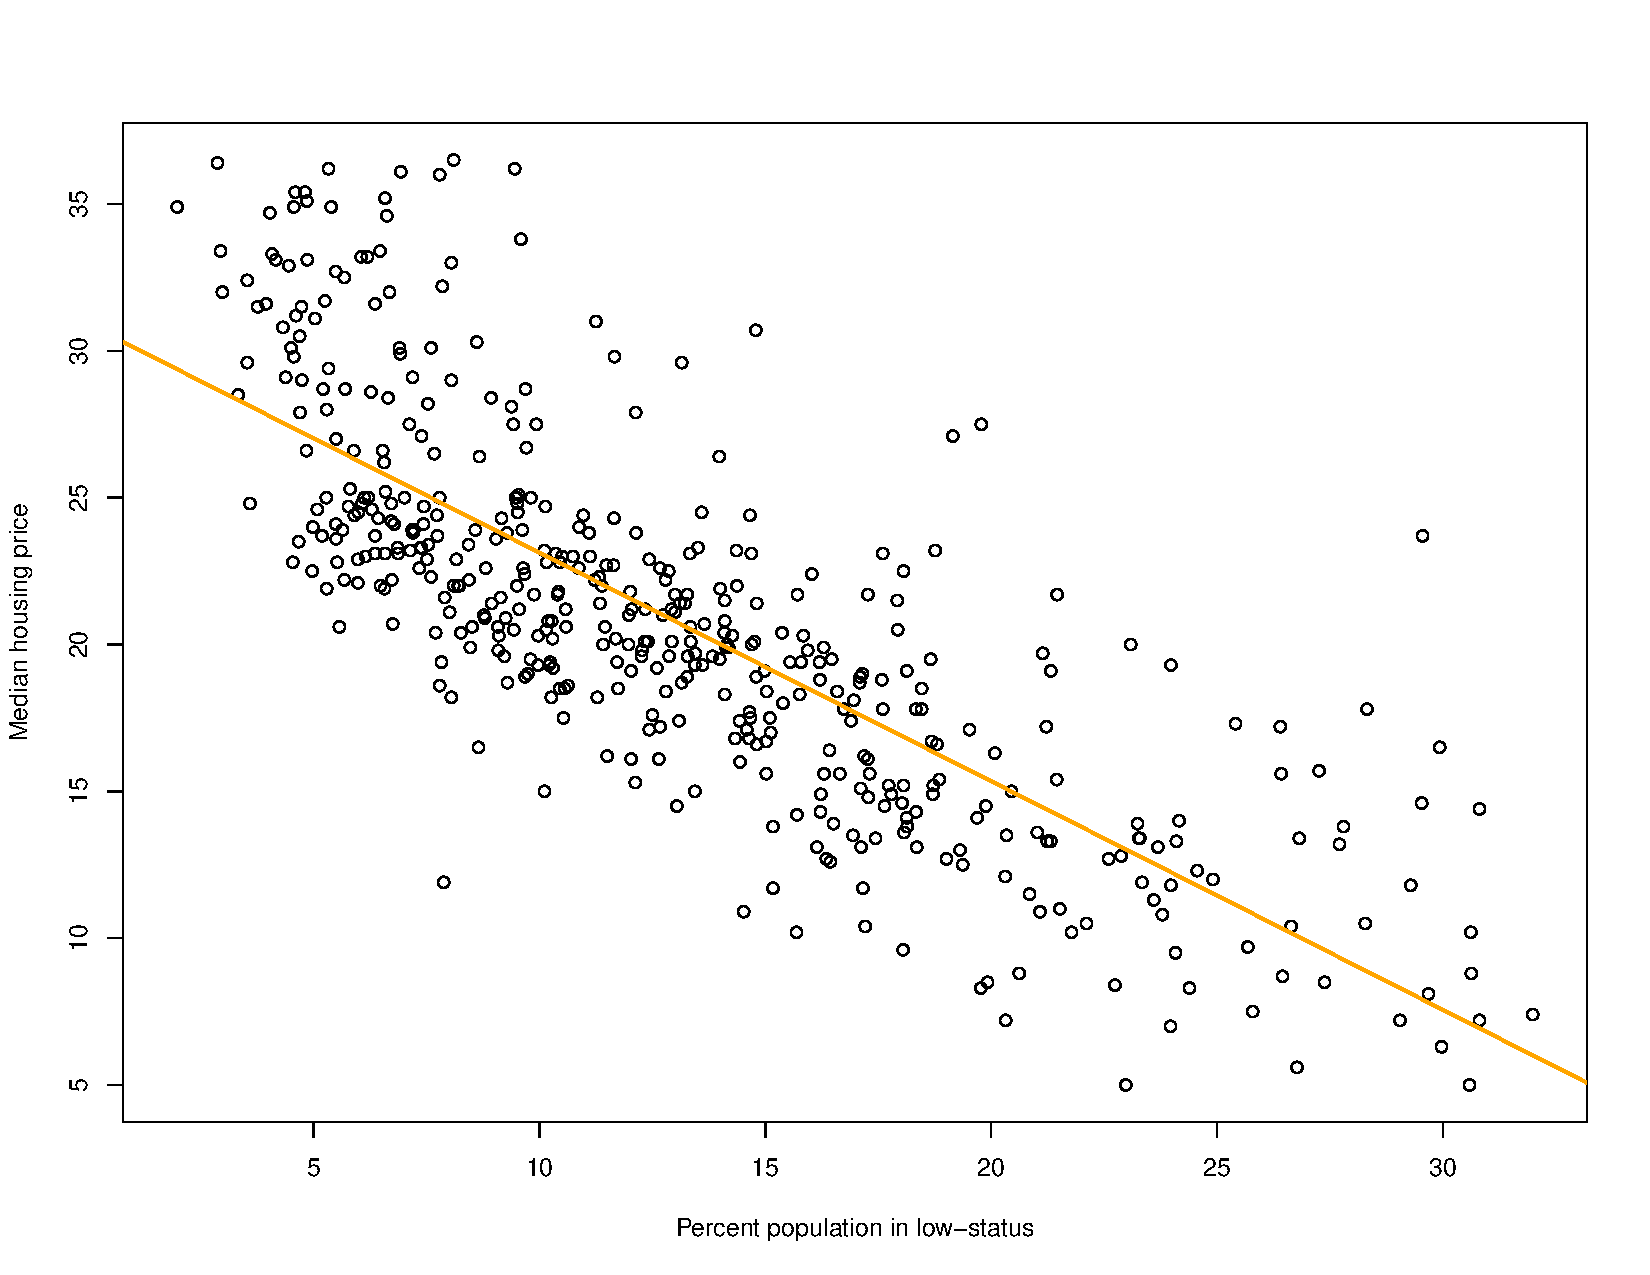
\includegraphics[width=0.65\linewidth]{medv-vs-lstat-simple-regression.pdf}
\end{figure}


%%%%%%%%%%%%%%%%%%%%%%%%%%%%%%%%%%%%%%%%%%%%%%%%%%%%%%%%%%%%%%%%%%%%%%%%%%%%%%%
{\large \bf Producing confidence intervals} \\
We can find the 95\% confidence intervals of our coefficients by calling R's 
confint() function:

\begin{verbatim}
> confint(lm.fit)
                 2.5 %     97.5 %
(Intercept) 30.0966007 31.7306978
lstat       -0.8344623 -0.7224984
\end{verbatim}

Also prediction intervals for lstat values 5, 10, and 15:

\begin{verbatim}
> predict(lm.fit, data.frame(lstat=c(5, 10, 15)),
+         interval="confidence")
       fit      lwr      upr
1 27.02125 26.44070 27.60180
2 23.12885 22.72485 23.53284
3 19.23644 18.85424 19.61865
\end{verbatim}

This tells us that for a location where about 10 percent of the population that
is of lower status, the median value for housing should be between $[22.72, 23.53]$
Similar predictions can be found for any value within the plotted bounds of the graphs
above. Otherwise predictions may not be accurate due to extrapolation.


\pagebreak

{\large \bf Diagnostic plots}
\begin{figure}[!ht]
  \centering
  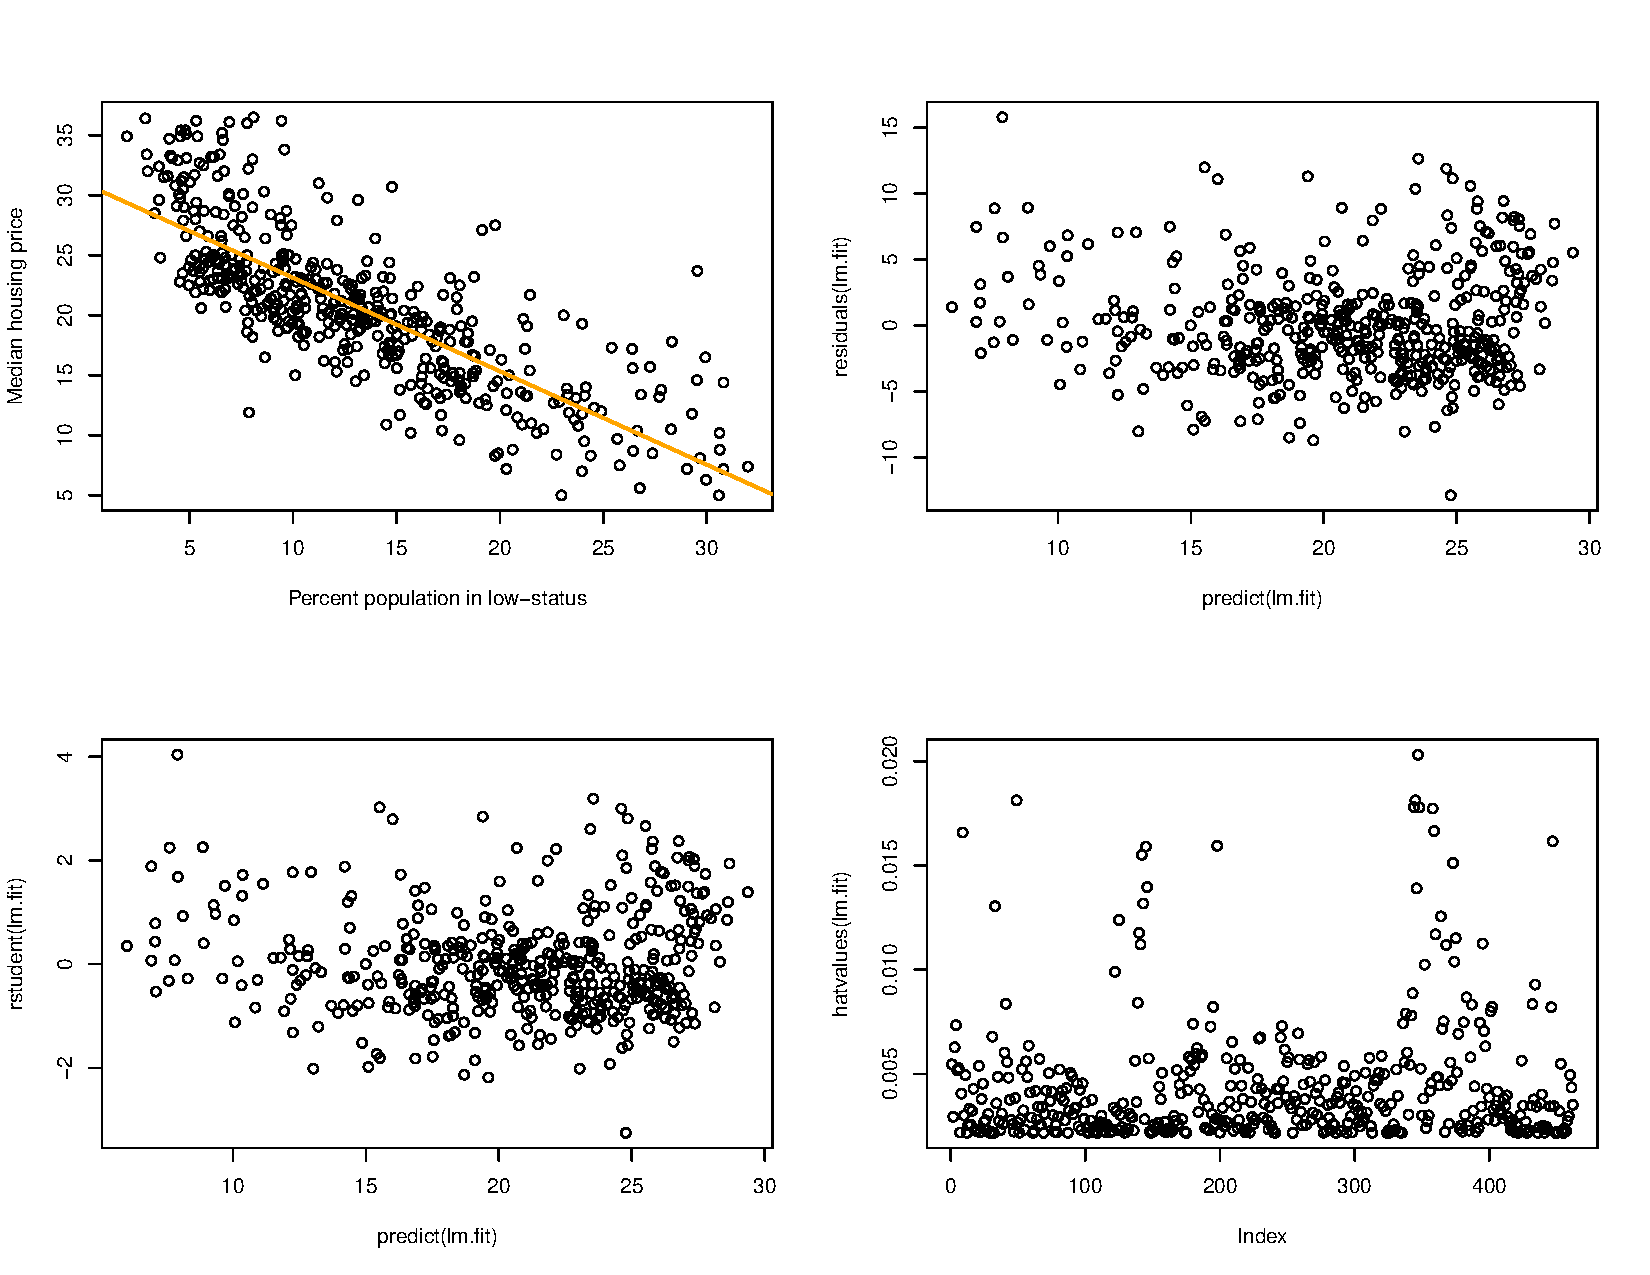
\includegraphics[width=1.00\linewidth]{diagnostic-plots.pdf}
\end{figure}

All code for plots and calculations can be found in 'simple-linear-regression.R'

\end{document}
